\documentclass[conference]{IEEEtran}
\IEEEoverridecommandlockouts
\usepackage{cite}
\usepackage{url}
\usepackage{seqsplit}
\usepackage{subcaption}
\usepackage{amsmath,amssymb,amsfonts}
\usepackage{graphicx}
\usepackage{textcomp}
% \usepackage{xcolor}
\usepackage{kotex}
\usepackage{multicol}
\usepackage{multirow}
\usepackage{booktabs} 
\usepackage{makecell}
\usepackage{algorithm}
\usepackage{algpseudocode}

\hbadness=99999  % or any number >=10000
\vbadness=99999  % or any number >=10000
\hfuzz 20pt

\def\BibTeX{{\rm B\kern-.05em{\sc i\kern-.025em b}\kern-.08em
    T\kern-.1667em\lower.7ex\hbox{E}\kern-.125emX}}
\begin{document}

\title{Upstream Based Low Latency Autoscaling for Microservices\\}

\author{\IEEEauthorblockN{%1\textsuperscript{st} 
    Jaehong Lee, and Euiseong Seo}
\IEEEauthorblockA{\textit{Department of Software, Sungkyunkwan University} \\
% \textit{name of organization (of Aff.)}\\
Suwon, Republic of Korea \\
{\{tutu083, euiseong\}@skku.edu}}}

\maketitle


% ----------------------------------------------------------------------------

\begin{abstract}
    최근 레거시 시스템을 마이크로서비스 아키텍처로 전환하려는 많은 시도가 있습니다. Scalability는 시스템의 유연성을 높이는 마이크로서비스 아키텍처의 주요 기능 중 하나입니다. 마이크로서비스를 위한 container orchestrator로써 업계 표준인 Kubernetes는 horizontal pod autoscaler(HPA)이라는 scalability 기능을 제공합니다. 일정한 scrape 주기마다 polling을 통해 메트릭을 수집하는 HPA의 동작은 낮은 스케일링 성능을 야기합니다. scrape 주기를 줄이는 방법이 고려될 수 있지만 기존 polling 메커니즘의 구조적 한계를 완전히 극복하기 어렵고 잦은 polling은 무의미한 네트워크 리소스를 낭비합니다. 본 논문에서는 이러한 HPA의 한계를 극복하기 위한 새로운 방안으로 upstream based horizontal pod autoscaler(UHPA)를 제안합니다. UHPA는 각 노드에 배치된 UHPA Agent 데몬과 스케일링 결정을 담당하는 UHPA Controller 간의 상호작용을 upstream 구조로 전환하여 실시간 메트릭 정보 업데이트를 통해 스케일링 성능을 크게 향상시킵니다. 우리는 Kind로 구축한 Kubernetes 클러스터에 UHPA 컴포넌트들을 배포하고, 오픈 소스 벤치마크를 통한 엔드투엔드 성능 평가를 진행했습니다. UHPA는 무시할 수준의 리소스 사용으로 기존 HPA 대비 스케일링 성능을 크게 향상 시켜 높은 서비스 품질을 제공했습니다.

\end{abstract}

% ----------------------------------------------------------------------------

\begin{IEEEkeywords}
    microservices, horizontal autoscaling, kubernetes, resource management
\end{IEEEkeywords}

% ----------------------------------------------------------------------------

\section{Introduction}
% 배경
마이크로서비스 아키텍처는 최근 대형 애플리케이션의 효율적인 개발, 배포 및 운영을 위한 주요 패러다임으로 자리잡고 있습니다. 기존 모놀리식 기반 아키텍처와 달리 마이크로서비스 아키텍처는 경량 API\cite{RedHatMicroservices}를 통해 서로 통신하는 독립적인 서비스들의 모음입니다. CPU, 메모리 및 네트워크 트래픽과 같은 수요에 따라 특정 서비스만 확장하는 scalability는 시스템 안정성을 유지하기 위한 핵심 기능 중 하나이며 이를 통해 효율적인 클러스터 리소스 활용과 지속적인 서비스 제공을 보장합니다.

% 구체적인 주제 및 중요한 이유
Kubernetes\cite{KubernetesOfficial}는 컨테이너 오케스트레이션 도구의 업계 표준으로 컨테이너화된 애플리케이션의 배포, 확장 및 관리 자동화를 통해 인프라의 효율성과 신뢰성을 향상시킵니다. Kubernetes는 scalability을 위해 HPA\cite{KubernetesHPA}라는 자체 확장 전략을 제공합니다. HPA는 시스템 운영자가 설정한 CPU 및 메모리 임계값을 활용한 규칙 기반 반응형 자동 스케일링 방법입니다. HPA 컨트롤러는 현재 동작중인 pod의 메트릭 값과 임계값을 통해 현재 클러스터에 필요한 pod 수를 결정합니다. 메트릭이 정의된 임계값을 초과하면 HPA는 적절한 노드에 마이크로서비스를 확장합니다. 이를 통해 쿠버네티스의 애플리케이션은 동적인 상황에 빠르고 쉽게 대응할 수 있습니다. 하지만, 우리는 HPA에 대한 심도있는 분석을 통해 HPA의 polling 메커니즘이 갖는 두 가지 문제점을 발견했습니다. 첫째, configuration 최적화를 통해 스케일링 성능 향상시켰음에도 여전히 부족한 스케일링 성능을 보입니다. 둘째, 최적화로 인한 구성 요소 간의 과도하게 짧은 scrape 주기는 높은 시스템 부하를 일으키고 네트워크 리소스를 낭비합니다. 이러한 문제로 시스템의 신뢰도가 떨어지고 서비스 품질에 부정적인 영향을 끼칠 수 있습니다.

% 과거의 시도
Kubernetes의 스케일링 성능을 향상시키기 위한 여러 연구가 수행되었습니다. 워크로드의 특성에 따라 HPA의 scrape 주기를 조정하는 반응형 방법\cite{jiang2021fine}이 제안되었지만, HPA의 구조적 한계를 근본적으로 해결하지 못합니다. 워크로드와 관련된 메트릭 예측을 통해 사전에 스케일링 하는 방법\cite{dang2021deep}\cite{he2020novel}\cite{zhao2019research}은 반응형 방법 대비 준수한 성능을 보입니다. 하지만, 검증에 활용된 제한된 실험 환경과 워크로드에 최적화된 방법은 실제 마이크로서비스간의 복잡한 관계를 반영하지 못합니다\cite{huye2023lifting}.

% 우리의 제안
우리는 기존 HPA 방식의 구조적 문제를 해결하기 위해 UHPA라는 새로운 upstream 기반의 horizontal pod autoscaler를 제안합니다. UHPA는 Agent와 Controller라는 두 가지 주요 구성 요소로부터 두 번의 의사 결정 프로세스를 통해 CPU 메트릭에 기반한 스케일링을 수행합니다. UHPA Agent는 각 노드에 데몬으로 배포되어 노드에 종속된 pod들의 CPU 사용량을 수집 및 관찰하고 제한된 환경 내에서 스케일링 여부를 1차로 결정합니다. 만약 스케일링이 필요하다고 판단되면, UHPA Agent는 UHPA Controller에게 해당 마이크로서비스의 스케일링 가능성을 검토하도록 요청합니다. UHPA Agent의 스케일링 검토 요청을 받은 후 UHPA Controller는 모든 UHPA Agent로부터 CPU 사용량을 수집합니다. 수집 된 CPU 사용량을 기반으로 해당 마이크로서비스의 전체 CPU 사용량을 계산하고 스케일링 필요성을 검토한 후, 적절한 pod 수를 Kubernetes API 서버를 통해 업데이트합니다. 실험을 통해 UHPA가 기존 HPA 대비 평균 20배 빠른 스케일링 성능을 보였습니다. 이러한 높은 스케일링 성능을 통해 오픈소스 벤치마크 애플리케이션을 활용한 엔드투엔드 실험에서 최대 93\%까지 응답률이 향상되었습니다. 또한 배포된 UHPA Agent와 Controller의 리소스 사용량은 무시할 수 있는 수준임을 확인했습니다.

% 목차 요약
이 논문의 나머지 부분은 다음과 같이 구성됩니다. 2절에서는 주로 Kubernetes의 기본 확장 전략과 한계에 대해 설명합니다. 3절에서는 우리의 새로운 제안에 대해 자세히 소개합니다. 4절에서는 UHPA의 성능을 평가하고 Kubernetes의 기본 확장 전략과 비교합니다. 마지막으로 5절에서는 결론과 함께 논문을 마무리합니다.

% ----------------------------------------------------------------------------

\section{Background and Motivation}
\label{sec:background and motivation}
Scalability는 마이크로서비스 아키텍처의 성공의 핵심 기능 중 하나로, 시스템의 유연성을 강화하고 서비스 품질을 향상시킵니다. 임계값 기반 자동 스케일링은 단순성과 높은 사용 용이성으로 널리 사용되고있습니다.

\subsection{Horizontal Pod Autoscaling of Kubernetes}
Kubernetes는 CNCF(Cloud Native Computing Foundation)의 주력 프로젝트로, 유연하고 효율적인 서비스 운영을 위해 많은 강력한 기능을 제공하는 컨테이너 오케스트레이터의 업계 표준입니다. HPA는 Kubernetes에서 마이크로서비스를 자동으로 확장하는 기능입니다. 그림 \ref{fig:hpa system design}은 HPA 워크플로우와 함께 Kubernetes에 구현된 시스템 아키텍처를 보여줍니다.

\begin{figure}[ht]
    \centerline{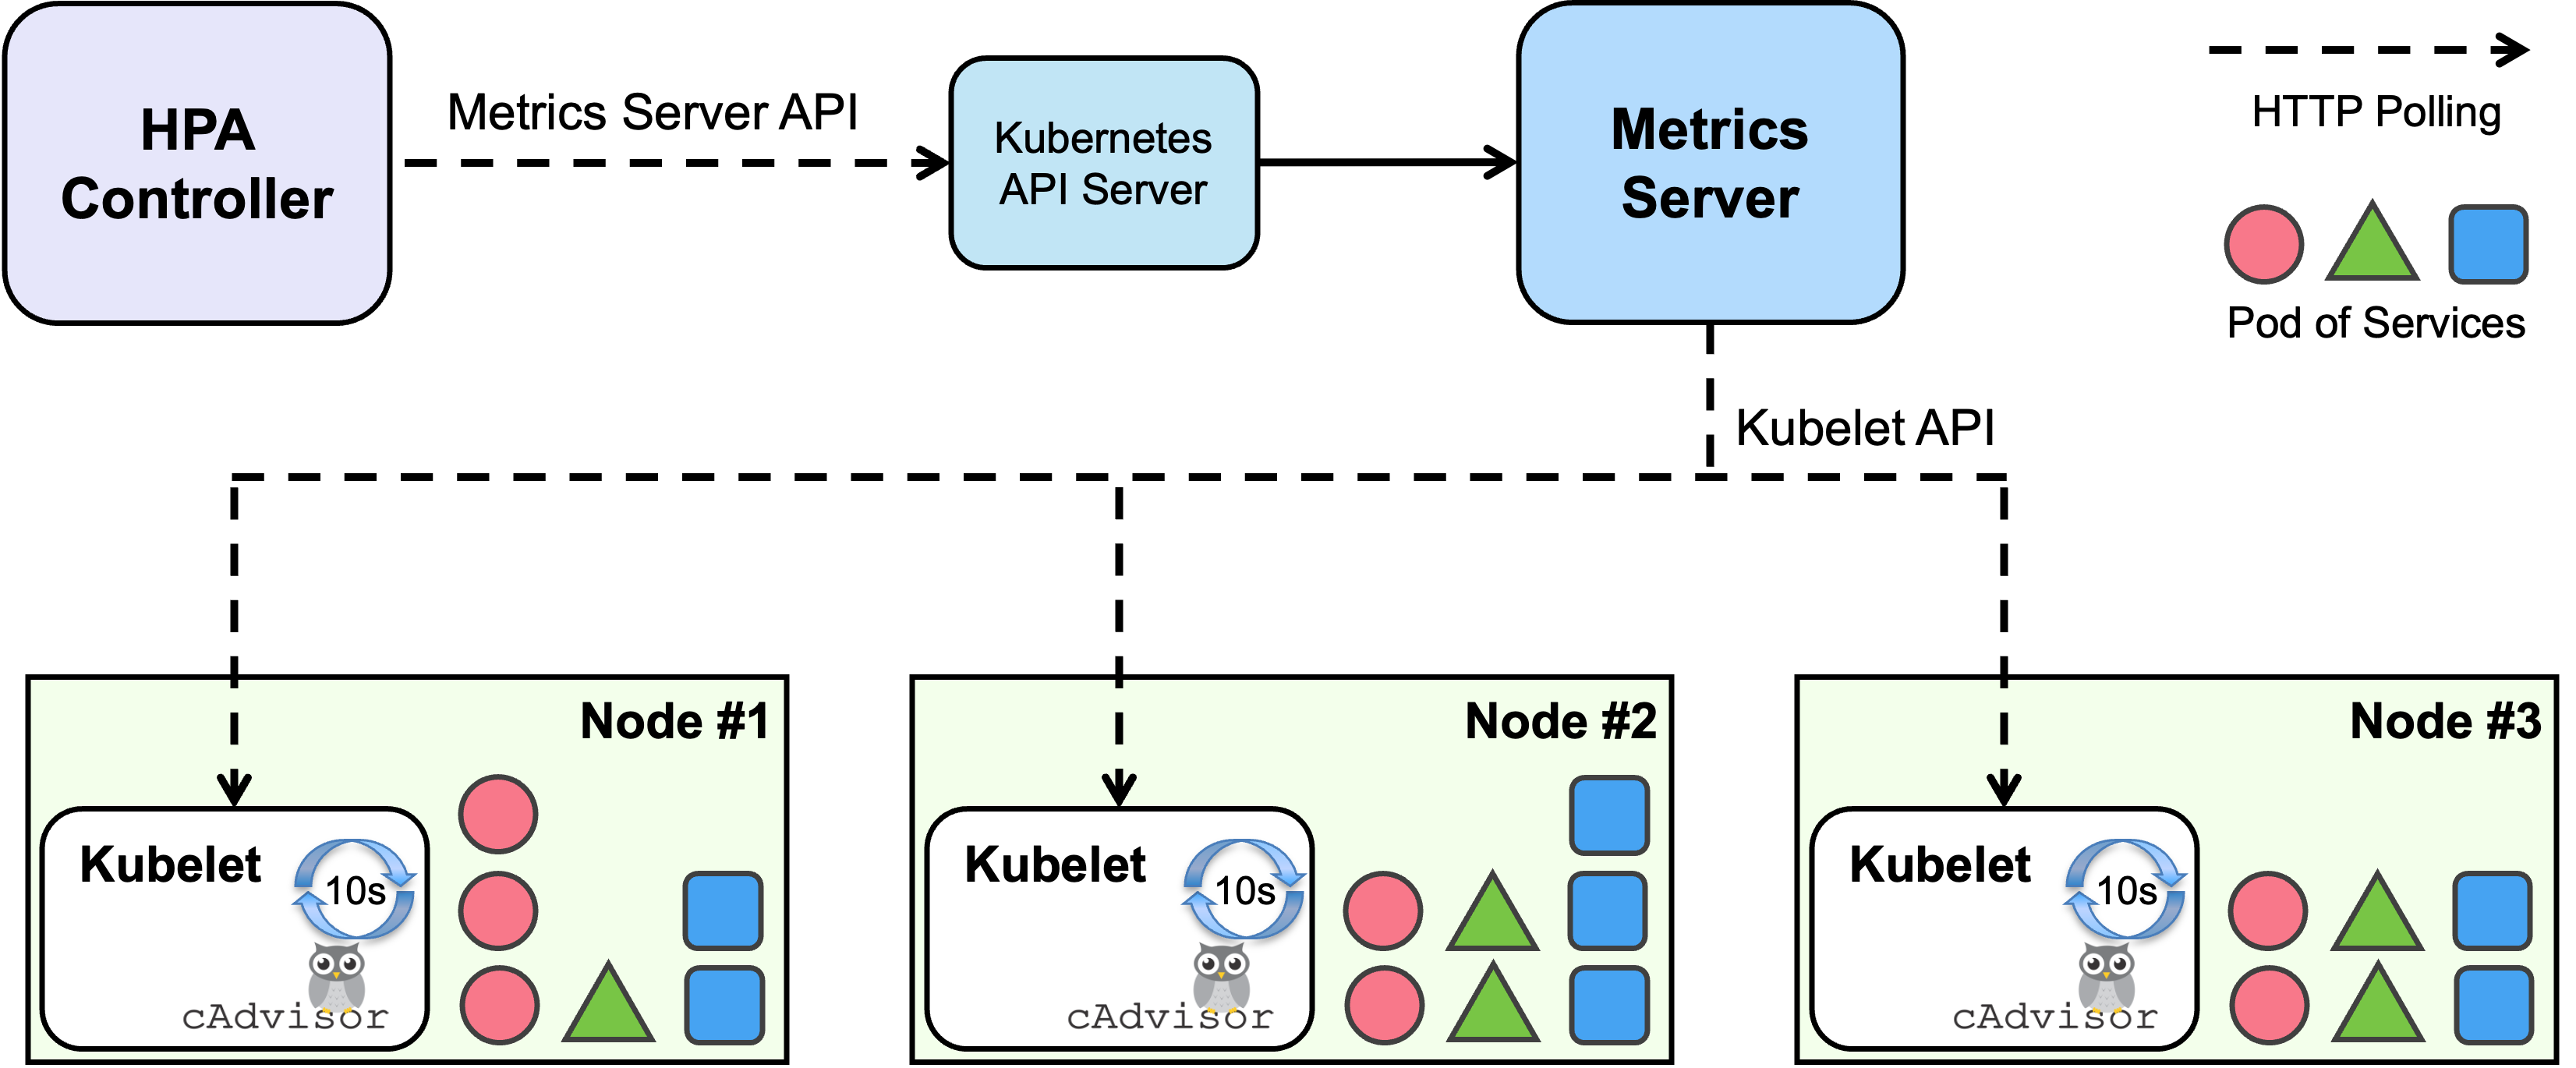
\includegraphics[width=8.5cm]{images/background/k8s_system_design.png}}
    \caption{HPA workflow}
    \label{fig:hpa system design}
\end{figure}

HPA는 Kubernetes에서 마이크로서비스를 구성하는 가장 작은 단위인 컨테이너 집합으로 구성된 pod의 CPU 사용량을 모니터링합니다. CPU 메트릭 수집 프로세스에는 Kubelet, Metrics-server 그리고 HPA 컨트롤러 총 세 가지 주요 구성 요소가 포함됩니다. 각 구성 요소는 polling 메커니즘을 통해 CPU 사용량을 수집합니다. 스케일링 동작을 위한 메트릭 수집은 총 3단계로 이루어집니다. 먼저 Kubelet은 cAdvisor\cite{cAdvisorGithub}에서 컨테이너에 관련된 모든 메트릭을 수집합니다. 이후 Metrics-server는 Kubelet의 REST API를 통해 CPU와 메모리 사용량을 수집하고 Kubernetes API 서버를 통해 노출합니다. 마지막으로 HPA 컨트롤러는 Kubernetes API 서버에게 필요한 CPU와 메모리 사용량 데이터를 요청합니다. 각 컴포넌트는 각자 설정된 scrape 주기를 기준으로 polling을 통해 메트릭을 수집합니다.

\begin{align}
    \label{eq:HPA desired replicas}
    \text{DesReplicas} = \left\lceil \text{CurReplicas} \times \left( \frac{\text{Total CPU Usage}}{\text{Target CPU Usage}} \right) \right\rceil
\end{align}

수집 과정에서 HPA 컨트롤러는 마이크로서비스를 구성하는 전체 pod의 현재 CPU 사용량과 시스템 운영자가 지정한 임계값을 기반으로 필요한 pod replica 수를 결정합니다\cite{KubernetesHPA}. 수식 \ref{eq:HPA desired replicas}은 HPA 컨트롤러에서 사용하는 공식을 나타냅니다. 필요한 replica 수인 DesReplicas는 총 CPU 사용량과 목표 CPU 사용량의 비율을 현재 replica 수인 CurReplicas에 곱하여 계산됩니다. 예를 들어 두 개의 pod로 구성된 마이크로서비스의 목표 CPU 사용률이 80\%이고, 현재 평균 CPU 사용률이 100\%인 경우 HPA 컨트롤러는 pod를 하나 추가해 총 세 개의 pod를 구성합니다. 이를 통해 해당 마이크로서비스의 CPU 사용률이 약 66.6\%로 감소하여 목표 CPU 사용률 보다 낮아집니다.


\subsection{Limitation of HPA}
우리는 HPA에 대한 다양한 실험과 소스 코드 분석을 통해, polling 메커니즘이 높은 스케일링 지연을 유발하고 클러스터 운영에 비효율적인 구조임을 확인했습니다. 특히, HPA의 기본 정책은 확장 시간이 길고 속도가 느린 문제로 낮은 QoS를 초래합니다\cite{huo2023high}.

\begin{table}[tb]
    \caption{Scrape interval of each component}
    \begin{center}
        \begin{tabular}{|c|c|c|}
            \hline
            \cline{2-3}
            \textbf{Component} & \textbf{{Default(s)}} & {\textbf{Optimal(s)}} \\
            \hline
            Kubelet            & 10                    & 10                    \\
            \hline
            Metrics-server     & 60                    & 15                    \\
            \hline
            HPA Controller     & 15                    & 1                     \\
            \hline
        \end{tabular}
        \label{tab:scrape interval of each component}
    \end{center}
\end{table}

성능 비교군을 위해, 표 \ref{tab:scrape interval of each component}에 명시된 scrape 주기를 적용한 기본 모드와 최적화 모드에서의 스케일링 성능을 측정했습니다. Kubelet은 cAdvisor를 통해 cgroup에서 CPU 관련 메트릭을 수집하며, "housekeeping\_interval"이라는 scrape 주기를 10초로 설정합니다. 이 설정은 시스템 상 변경할 수 없기 때문에 모든 실험에서 동일 값을 사용합니다. Metrics-server는 HTTP 요청을 통해 각 노드의 Kubelet에서 메트릭을 수집하며, 기본적으로 60초마다 데이터를 가져옵니다. 이 수집 주기는 "metric-resolution" 파라미터를 조정함으로써 변경이 가능하며, 최적화 모드에서는 공식 문서에서 권장하는 15초의 최소값을 사용합니다\cite{metrics-server-FAQ}. HPA Controller는 기본 scrape 주기로 15초를 설정하였으며, 최적화 모드에서는 "horizontal-pod-autoscaler-sync-period" 값을 1초로 조정하여 실험을 수행했습니다.

\begin{figure}[tb]
    \centering{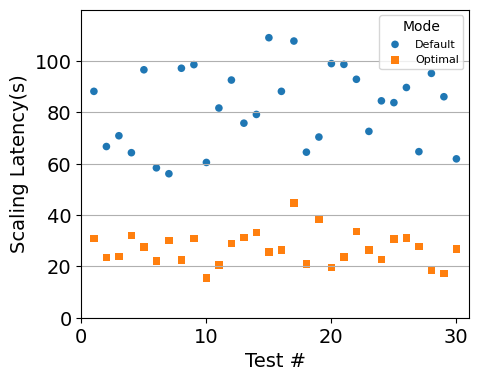
\includegraphics[width=5.7cm]{images/background/scaling_latency_without_UHPA.png}}
    \centering{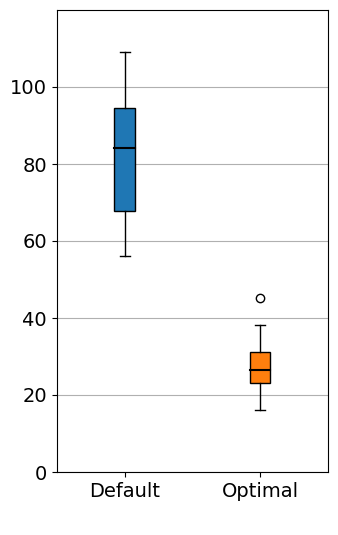
\includegraphics[width=2.8cm]{images/background/scaling_latency_boxplot_without_UHPA.png}}
    \caption{Scaling latency according to scrape interval}
    \label{fig:scaling time}
\end{figure}

그림 \ref{fig:scaling time}은 각 모드에서 마이크로서비스의 CPU 사용량이 임계값을 초과한 후 pod가 확장되기까지의 시간을 나타냅니다. 기본 모드는 56초에서 109초까지 넓은 분포를 보이며, 평균적으로 스케일링 완료까지 약 82초가 소요됩니다. 반면, 최적화 모드에서는 스케일링이 평균적으로 27초에 이루어지며, 16초에서 45초 사이의 변동 폭을 보였습니다. 우리는 이러한 실험 결과를 통해 HPA의 두 가지 문제점을 발견할 수 있었습니다.\\

\noindent\textbf{1) 스케일링 성능 개선을 위해 Scrape 주기를 줄이는 방식에는 한계가 있습니다.} Scrape 주기 조절을 통한 스케일링 성능 향상 실험에서, 메트릭 수집의 최적화 설정에도 불구하고 상당한 시간 지연이 발견되었습니다. 최적화 모드가 기본 모드에 비해 약 70\% 성능 향상을 보였지만, 평균 약 27초의 지연은 여전히 느린 편입니다. 각 컴포넌트의 Scrape 주기는 기본적으로 메트릭 수집 지연을 유발하며, 최악의 상황에서는 이러한 지연이 각 Scrape 주기의 총합이 됩니다. 또한, Metrics-server는 최근에 수집된 두 메트릭 값(n, n-1)의 평균을 마이크로서비스의 현재 CPU 사용률로 사용합니다. 이렇게 전달된 CPU 사용률은 HPA 컨트롤러가 로드가 선형적으로 또는 급격하게 증가할 때 실제 CPU 사용량을 과소평가하게 되는 원인이 됩니다. 이러한 이유로 실험 결과는 모든 컴포넌트의 scrape 주기의 합계보다 긴 지연 시간을 보여줍니다. 예를 들어, 그림 \ref{fig:scaling time}에서 최적화 모드의 결과 대부분은 각 컴포넌트의 scrape 주기(10초, 15초, 1초)의 합인 26초보다 높습니다.\\

\noindent\textbf{2) 구성 요소 간의 다중 polling 구조는 클러스터 운영에 비효율적입니다.}
Scrape 주기를 짧게 줄이면 Metrics-server가 각 노드의 Kubelet에 보내는 HTTP 요청이 증가하여 클러스터 내 과도한 네트워크 트래픽을 유발할 수 있습니다. 이와 함께, Kubernetes API 서버를 통해 Metrics-server로부터 메트릭을 수집하는 HPA Controller의 짧은 polling 주기는 Kubernetes API 서버의 로드를 증가시킵니다. API 서버의 부하 증가와 지속적인 네트워크 트래픽은 전체 클러스터 성능 오버헤드의 원인이 될 수 있습니다\cite{ExpediaGroupTech2020}. 더욱이 스케일링이 필요 없는 상황에서도 불필요하게 잦은 메트릭 수집은 클러스터의 네트워크 리소스를 불필요하게 소모하게 만듭니다.

\subsection{Related Work}
우리는 Kubernetes에서 제공하는 자동 스케일링의 문제점과 한계를 분석했습니다. 이와 관련하여, 유사하게 문제를 분석하고 개선된 스케일링 성능을 제공할 수 있는 다양한 방법들이 제시되었습니다.
먼저, 워크로드 상태가 낮음, 중간, 높음에 따라 메트릭 수집 빈도를 조절하는 방법이 제안되었습니다\cite{jiang2021fine}. 이 방식은 워크로드의 특성에 따라 scrape 주기 변경을 통해 세분화된 스케일링을 기능을 제공합니다. 그러나, 이 방법은 우리의 최적화 모드 실험 결과에서 알아본 것처럼 여전히 HPA의 구조적인 한계를 극복하지 못합니다.

워크로드를 예측하고 동적으로 대응하는 방법 또한 제안되었습니다. ARIMA와 같은 통계 모델을 활용하면 워크로드 예측 시 좋은 성능을 보이며, 이를 통한 선제적 확장으로 서비스 품질을 향상시킬 수 있습니다\cite{he2020novel}\cite{zhao2019research}. 그러나 워크로드 데이터가 지속적으로 변화함에 따라 예측 정확도가 감소하고, 특히 변동성이 큰 워크로드에서 이러한 문제가 두드러집니다\cite{yunyun2022research}.

마지막으로, 기계 학습을 활용한 워크로드 예측 방법도 활발히 진행되고 있습니다\cite{dang2021deep}\cite{gan2021sage}. 기계 학습 모델은 일반적으로 시계열 분석에 기반한 워크로드 예측보다 더 우수한 성능을 보여줍니다\cite{shim2023predictive}. 하지만, 여전히 과거 데이터를 기반으로 학습하는 접근 방식은 자주 업데이트되는 마이크로서비스 아키텍처에 적합하지 않습니다. 또한, 실제 마이크로서비스 환경은 실험 환경보다 훨씬 더 복잡하기 때문에 학습을 위해 설정한 다양한 가정들은 실제 마이크로서비스 아키텍처를 완전히 반영하지 못합니다\cite{huye2023lifting}.

이 문제를 해결하기 위해, 우리는 새로운 업스트림 기반 horizontal pod autoscaler인 UHPA를 제안합니다. UHPA는 UHPA Controller와 각 노드에 배포된 UHPA Agent 데몬을 활용한 2단계 결정 메커니즘을 사용합니다. UHPA의 목표는 신속한 의사결정을 가능하게 하여 스케일링 성능을 향상 시킴으로써 시스템의 신뢰성을 높이고, 불필요한 네트워크 트래픽을 최소화하는 것입니다.


% ---------------------------------------------------------------- ------------


\section{Upstream Based Horizontal Pod Autoscaler}
\subsection{System Overview}

\begin{figure}[tb]
    \centerline{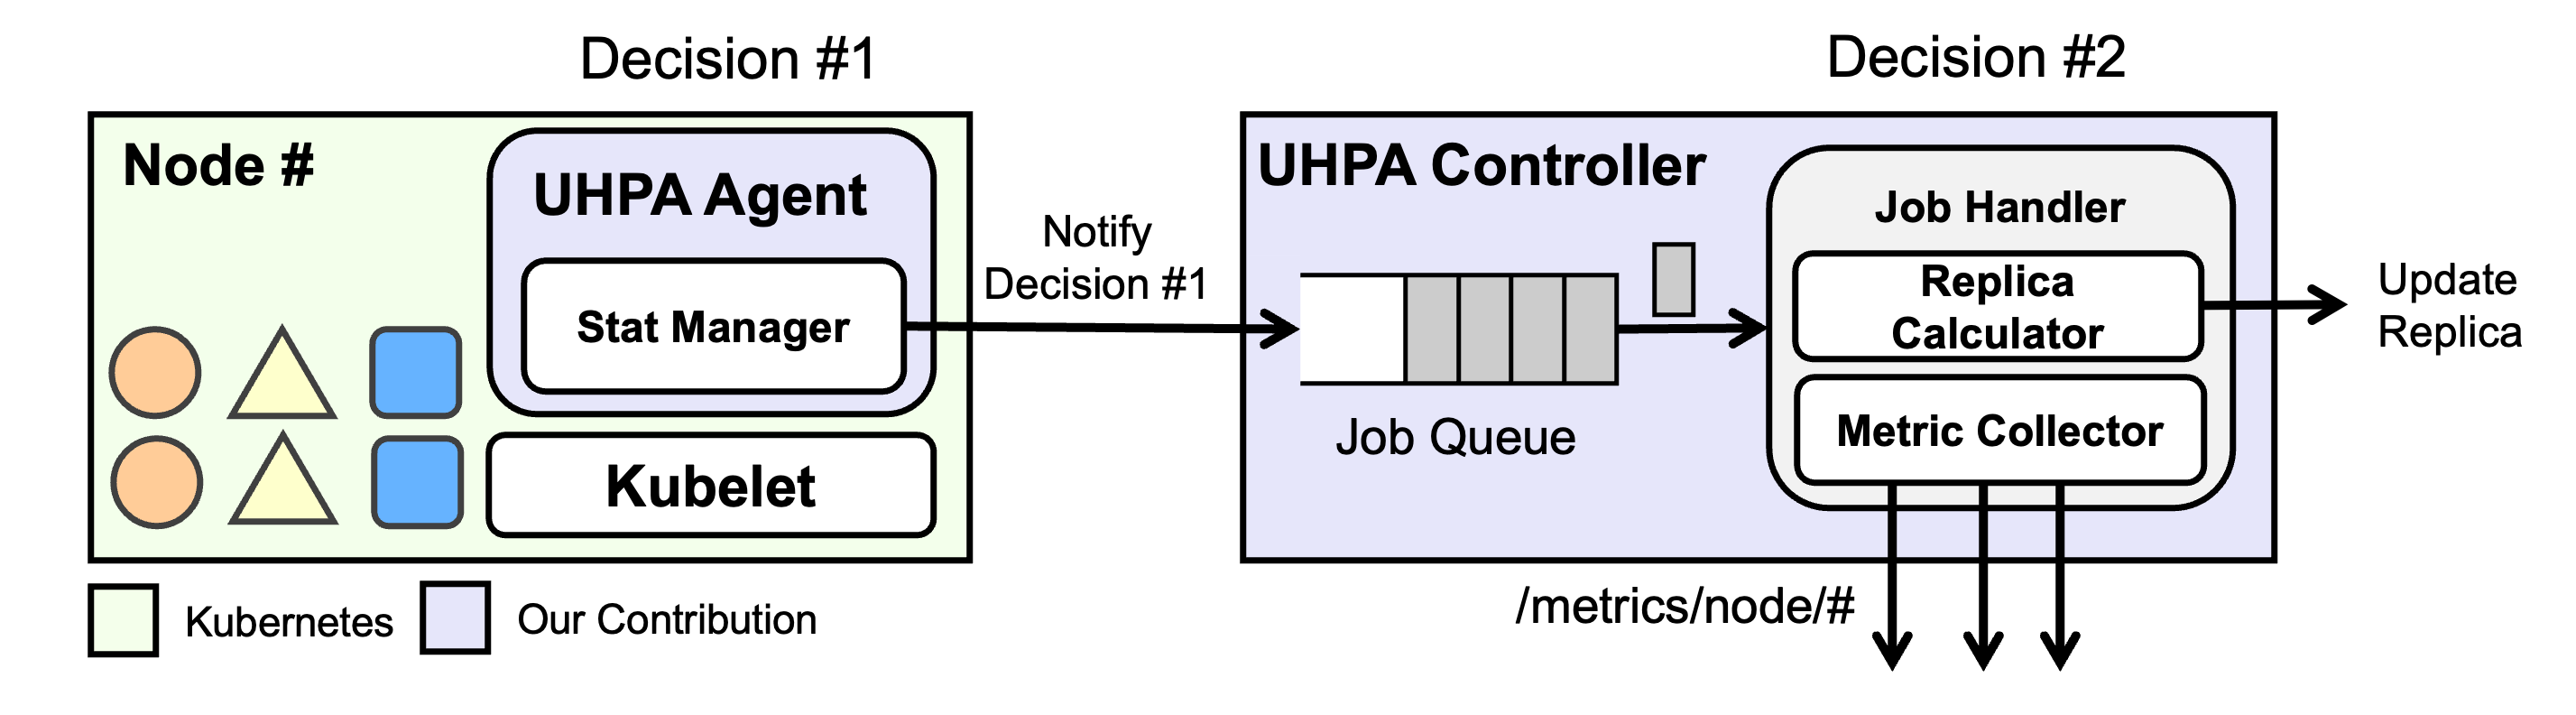
\includegraphics[width=8.5cm]{images/approch/uhpa_system_design.png}}
    \caption{System design of UHPA}
    \label{fig:uhpa system design}
\end{figure}

그림 \ref{fig:uhpa system design}은 UHPA의 두 가지 주요 구성 요소인 Agent와 Controller를 중심으로한 시스템 아키텍처를 나타냅니다. 클러스터 내 모든 Worker 노드에 배포된 UHPA Agent는 Stat Manager를 통해 Pod의 CPU 사용 데이터를 정기적으로 수집합니다. HPA가 컴포넌트 간 주기적인 polling을 통해 메트릭을 수집하고 HPA 컨트롤러에 의해 최종 스케일링 여부를 결정하는 반면, UHPA는 Agent가 자체 노드에 배포된 pod의 CPU 사용량을 기반으로 1차 스케일링 결정을 내리고 이를 Controller에 알리는 업스트림 방식을 사용합니다. 이 접근법은 시스템 운영자가 설정한 임계값을 감지하는 성능을 크게 향상시킵니다.

UHPA Agent는 UHPA Controller와 독점적으로 상호 작용합니다. 이는 시스템 구조를 단순화하고 UHPA 컴포넌트 간의 데이터 동기화를 위한 것입니다. 따라서 UHPA Controller는 Kubernetes API 서버를 통해 스케일링에 관한 정보를 수집하고, 이를 모든 UHPA 에이전트에 제공하는 역할을 담당합니다. 또한, UHPA Controller는 UHPA Agent의 1차 결정을 검토하고 최종 스케일링 여부를 결정합니다. 이러한 효율적인 2단계 상호 작용 모델은 HPA의 3단계 상호 작용 모델에서 발생하는 구조적 비효율성을 개선합니다.

\subsection{Lightweight CPU Metric Collection}
마이크로서비스 아키텍처의 핵심 장점은 독립적인 배포와 느슨한 결합입니다\cite{MicroservicesIO}. 이러한 이점을 극대화하기 대부분의 마이크로서비스는 상태 데이터를 저장하지 않는 stateless 서비스로 설계하여 배포, 확장 및 교체를 단순화합니다\cite{gan2019open}\cite{AWSStatefulActorServices2023}. 스토리지 서비스, 롤링 업데이트, 순차적 배포 등 몇 가지 특별한 경우를 제외하고, stateless 서비스는 마이크로서비스의 기본 유형입니다\cite{KubernetesStatefulSet2023}. 이러한 유형의 서비스는 CPU 메트릭의 영향을 크게 받습니다.

OS-level metrics CPU and memory usage are more highly correlated with workloads in microservice architecture\cite{luo2022power} and most stateless microservices are more affected by CPU usage than memory. Although HPA provides memory-based autoscaling, this feature is particularly tailored to specific cases like such as databases, caching services, which are less sensitive to scaling performance. With tracking frameworks like Jaeger\cite{JaegerTracing}, methods utilizing application-level metrics, such as response time and input request rate, have been proposed\cite{he2020novel}\cite{pramesti2022autoscaling}. However, these metrics can be influenced by unexpected external system environments, and their limited experimental settings do not accurately represent industrial microservice architectures or workloads\cite{huye2023lifting}. On the other hand, OS-level metrics are less affected by the external environments. Informed by this research, UHPA decided on CPU usage, a simple but powerful and practical OS-level metric, as the scaling metric.

Kubelet deployed on each node collects and exports various information related to the network and disk, as well as the CPU and memory usage of all deployed containers through the built-in cAdvisor. The housekeeping-interval, which is the scrape interval, is fixed to 10 seconds. This is because cAdvisor collects a large amount of information related to all containers running on the node, so if the scrape interval is too shortened, it may result in high CPU usage\cite{KubecostcAdvisor}. To solve this issue, we adopted a lightweight strategy that collects only CPU metric of the target microservices registered by HorizontalPodAutoscaler of Kubernetes as follows.

\begin{enumerate}
    \item All UHPA Agents periodically obtain target microservices list and scaling information  through UHPA Controller.

    \item UHPA Agent finds and stores the path of each container under "/sys/fs/cgroup/" where CPU metrics are stored through container IDs in the information.

    \item Every second, UHPA Agent reads CPU metrics from each container's path and calculates the CPU usage rate based on "requests.cpu" values in the description of pods.
\end{enumerate}

We use the 5-second average data to ignore cases of unusual spiky workloads in a very short period of time.


\subsection{Two-step Decision Mechanism}
As discussed in session II, Kubernetes' HPA can not raise scaling performance above a certain level due to the structural limitation. In addition, the main components keep communicating each other even in stable workloads where do not require scaling. We propose a two-step decision mechanism for designing upstream based low latency autoscaling to overcome the limitation of the polling mechanism. The two-step decision mechanism guarantees not only high scaling performance but also low system overhead by reducing unnecessary network traffic under stable workloads.

The first decision is made by UHPA Agent. UHPA Agent continuously collects CPU metrics of pods deployed on the node, calculates the CPU usage rate, and compares it with each target threshold. If the CPU usage rate of subset pods of a microservice is higher than the threshold, UHPA Agent makes the first decision to notify UHPA Controller of the microservice. Unlike the existing HPA's polling method, the method making preemptive decision in the node can ensure faster detection performance. However, this decision does not be the right for the entire cluster. Kubernetes distributes traffic coming into microservices to pods using an Iptables-based random method. This method is not fair traffic distribution like the commonly known round-robin, which can cause traffic to be concentrated on certain pods. Therefore, inferring the traffic of the entire microservice by observing only the subset pods deployed on one specific node can lead to underestimate or overestimate CPU usage. It means it is inevitable to collect metrics from all UHPA Agents deployed each node.

The second decision is made by UHPA Controller. When UHPA Controller receives a notification from UHPA Agent, it requests the CPU usage of that microservice from all UHPA Agents and recalculates the total usage rate. If the CPU usage rate is higher than the threshold, UHPA Controller makes a final decision by notifying the Kubernetes API server that the microservice needs scaling.
Under stable workloads, if there is no notification from UHPA Agent, the UHPA Controller no longer interacts unnecessarily. Next, we give a detailed explanation of each decision based on the two algorithms. \\

\begin{algorithm}[tb]
    \caption{First decision procedure in UHPA Agent}
    \begin{algorithmic}[1]
        \While{\textbf{true}}
        \State $l \gets \text{an empty list}$
        \For{\textbf{each} $int\_MS$ \textbf{in} $int\_MSs$}
        \State $stcr \gets 0$
        \For{\textbf{each} $pod$ \textbf{in} $int\_MS\rightarrow\text{pods}$}
        \State $stcr \gets t + \Call{CalCPURate}{pod}$
        \EndFor
        \State $sacr \gets stcr / \Call{Length}{int\_MS\rightarrow\text{pods}}$
        \If{$sacr > int\_MS\rightarrow\text{threshold}$}
        \State \Call{Append}{$l, int\_MS$}
        \EndIf
        \EndFor
        \If{$\Call{Length}{l} > 0$}
        \State \Call{NotifyToController}{$l$}
        \EndIf
        \State sleep(1)
        \EndWhile
    \end{algorithmic}
    \label{alg:agent}
\end{algorithm}

\begin{algorithm}[tb]
    \caption{Final decision procedure in UHPA Controller}
    \begin{algorithmic}[1]
        \While{\textbf{true}}
        \If{\Call{IsQueueEmpty}}
        \State sleep(1)
        \State \textbf{continue}
        \EndIf
        \State $j \gets \Call{Dequeue}{Job}$
        \State $CSList \gets \Call{GetCPUStatFromAgents}{j\rightarrow\text{MS}}$
        \State $N \gets 0$
        \State $tcr \gets 0$
        \For{\textbf{each} $CS$ \textbf{in} $CSList$}
        \If{\Call{IsNotEmpty}{$CS$}}
        \State $tcr \gets tcr + \Call{CalCPURate}{CS}$
        \State $N \gets N + 1$
        \EndIf
        \EndFor
        \State $acr \gets tcr / N$
        \If{$acr > j\rightarrow\text{threshold}$}
        \State \Call{DoScale}{$j\rightarrow\text{MS}$}
        \EndIf
        \EndWhile
    \end{algorithmic}
    \label{alg:controller}
\end{algorithm}

\noindent\textbf{\textit{1) First Decision by UHPA Agent}}
\par Alg. \ref{alg:agent} shows how the UHPA Agent, deployed on each node as a DaemonSet of kubernetes, make the first decision. It continuously collects the CPU usage for scalable microservice pods. Since two or more pods of a microservice can be deployed on each node, we use the average CPU usage rate of subset pods(sacr) divided by the number of subset pods from the total cpu usage rate(stcr) as our decision metric(line 5-8). Eq. \ref{eq:cpu rate} shows the formula for calculating the average CPU Usage rate for N pods, and this method is the same as the method used in HPA. Next, the UHPA Agent compares the average CPU usage rate with the target threshold of each microservice, and informs UHPA controller, if there are microservices with the average CPU usage rate higher than the threshold(line 9-14). This process repeats every second. \\

\begin{align}
    \text{rate(\%)} = {\frac{\sum_{i=1}^{N} \left( \frac{\text{Current CPU Usage}_i}{\text{CPU Requests}_i} \right)}{N} \times 100}
    \label{eq:cpu rate}
\end{align}

\noindent\textbf{\textit{2) Second Decision by UHPA Controller}}
\par Alg. \ref{alg:controller} describes how the UHPA Controller handles notifications received from UHPA agents and makes final scaling decisions. First, scaling notifications received from UHPA Agents are inserted into the job queue, and processed sequentially through dequeuing. Next, CPU usage of all pods constituting the target microservice is collected from all UHPA Agents(line 7). With the CPU usage set collected from each UHPA agent, UHPA Controller calculates the average CPU usage rate(acr) divided by the number of pods(N) from the total cpu usage rate(tcr)(line 10-16). Finally, UHPA Controller compares the average CPU usage rate to the target threshold of the microservice again, and if the average CPU usage rate is higher than the threshold, Eq. \ref{eq:HPA desired replicas} is used to calculate the number of pods required and update the calculated pod replica(s) through the Kubernetes API server.


% ----------------------------------------------------------------------------


\section{Evaluation}
우리의 제안을 평가하기 위해 Kind\cite{KindK8s}에서 생성한 로컬 Kubernetes 클러스터에 UHPA Agent 및 Controller 배포합니다. UHPA Agent Kubernetes의 DaemonSet으로 각 노드에 배포되므로 UHPA Agent수와 동일합니다. 클러스터에 HPA Controller는 Kubernetes의 Deployment 형태로 하나만 배포됩니다. 결과에 영향을 미칠 수 있는 외부 요인의 영향을 제거하기 위해 모든 테스트는 Kubernetes 클러스터 생성부터 시작됩니다. 실험 결과를 HPA의 두 모드와 비교하여 UHPA의 성능을 검증합니다.

\begin{figure}[tb]
    \centering{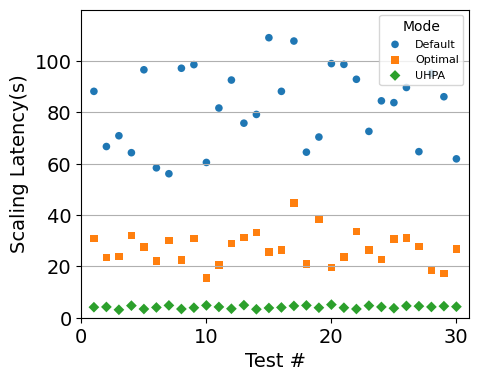
\includegraphics[width=5.7cm]{images/evaluation/scaling_latency_with_UHPA.png}}
    \centering{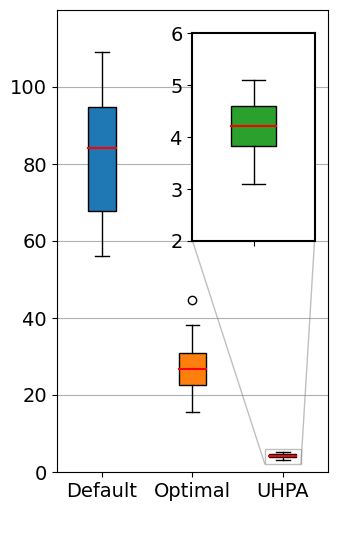
\includegraphics[width=2.8cm]{images/evaluation/scaling_latency_boxplot_with_UHPA.png}}
    \caption{Scaling latency comparison}
    \label{fig:scaling latency comparison}
\end{figure}

\subsection{Latency Analysis}
UHPA의 지연시간을 측정하기 위해 세개의 워커 노드와 마스터 노드에 UHPA 컴포넌트들을 배포하고 각 구간에서 발생하는 Latency를 체크했습니다. 우리는 nginx 애플리케이션을 사용하여 설정한 threshold인 CPU usage rate 80\%을 감지한 후 pod가 생성된 후 Ready 상태에 이를 때까지 발생되는 지연 시간을 평가했습니다. 실험은 총 20번 진행되었습니다.


첫 번째 구간은 목표 임계값을 충분히 초과하는 트래픽이 부과되는 시점과 UHPA 에이전트가 이를 감지하고 첫 번째 스케일링 결정을 UHPA 컨트롤러로 보내는 지연 시간입니다. 이 구간에서 UHPA는 평균 3.2초, 95번째 백분위수에서 3.6초의 지연 시간을 갖습니다. UHPA Agent는 매초마다 CPU 메트릭을 읽기 때문에 트래픽에 민감하게 반응할 수 있습니다. 따라서 짧은 탐지 시간을 보장합니다. 두 번째 구간은 UHPA Controller가 UHPA Agent로 부터 notification을 받고 각 UHPA Agent로 부터 CPU usage를 수집하고 Kubernetes API server에 pod replica를 업데이를 하는 구간이다. 해당 구간은 평균 0.5, 95 백분위수 0.9 초라는 아주 짧은 Latency를 가진다. UHPA Controller는 병렬 처리 기반으로 모든 UHPA 에이전트의 CPU 사용량을 수집하므로, 지연 시간은 마지막 응답을 보내는 노드의 영향만 받기 때문에 노드 수는 전체 지연 시간에 큰 영향을 미치지 않습니다. 마지막 세 번째 섹션은 실제 pod가 특정 노드에 배포되고 준비 상태에 도달하여 사용 가능해질 때까지입니다. 마지막 세 번째 섹션에서 발생하는 Latency는 UHPA Controller가 Kubernetes API server에 pod replica 업데이트를 요청한 후의 Latency이므로 UHPA의 실제 성능과는 관련이 없습니다. \ref{fig:scaling latency comparison}는 HPA와 UHPA의 두 가지 모드 간의 scaling 성능을 비교한 결과를 보여줍니다.  UHPA는 HPA 보다 월등히 빠른 성능과  낮은 지연시간 스펙트럼을 보여줍니다.

우리는 본 실험을 통해서 평균 실제 UHPA 동작에 의해서만 발생하는 latency가 3.7초, 95 백분위수 4.5초 수준임을 확인했다. 이러한 성능 향상은 HPA의 넓은 성능 스펙트럼 구간을 약 1초로 줄였으며 대부분의 경우 5초안에 스케일링이 요청이 완료되는 보장성을 제공합니다.


% \begin{table}[tb]
%     \caption{Scaling performance comparison}
%     \begin{center}
%         \begin{tabular}{|c|c|c|c|}
%             \hline
%             \multicolumn{4}{|c|}{\textbf{Scaling Latency(s)}}                                          \\
%             \cline{1-4}
%             \hline
%             \textbf{} & \textbf{Default} & \textbf{Optimal} & \textbf{UHPA} \\
%             \hline
%             Average   & 81                        & 27                        & 4                      \\
%             \hline
%             Min       & 51                        & 16                        & 3                      \\
%             \hline
%             Max       & 109                       & 45                        & 5                      \\
%             \hline
%             Perc.95   & 108                       & 41                        & 5                      \\
%             \hline
%         \end{tabular}
%         \label{tab:scaling_performance_comparison}
%     \end{center}
% \end{table}


\subsection{Performance Comparison}

\begin{figure}[tb]
    \centering
    {\includegraphics[width=8.8cm]{images/evaluation/social-netwrok.png}}
    \caption{Social network application structure}
    \label{fig:social network}
\end{figure}


우리는 UHPA의 성능과 실용성을 검증하기 위해 엔드 투 엔드 성능 테스트를 수행했습니다. 테스트의 주요 목적은 UHPA가 HPA보다 비해 얼마나 빨리 pod를 확장시키고 이러한 스케일링 성능이 전체 시스템 QoS에 어떤 영향을 끼치는지를 이해하는 것입니다. 실험을 위해 Kind로 3개의 작업자 노드와 1개의 마스터 노드를 구성하고 UHPA 컴포넌트를 배포했습니다.

실험에서 모든 stateless 서비스의 target threshold인 CPU 사용률은 80\%로 설정하고 requests.cpu는 30m로 설정합니다. 모든 stateless 서비스의 최소 복제본 수는 1이고 최대 복제본 수는 제한이 없습니다. 성능 비교를 위해 HPA의 두 모드와 UHPA를 가지고 동일한 실험을 진행합니다. 기본 모드와 최적 모드의 스크랩 간격 값은 Section \ref{sec:background and motivation}의 Table \ref{tab:scrape interval of each component} 에서 확인할 수 있습니다. 스케일링에 영향을 미치는 또 다른 요소로 limits.cpu가 있습니다. requests.cpu가 컨테이너가 보장받아야 할 CPU 리소스라면 limits.cpu는 컨테이너가 사용할 수 있는 최대 CPU 리소스 값입니다. 스케일링이 필요 시점에 limits.cpu값에 여유가 있다면 높은 시스템 신뢰성을 확보할 수 있습니다. 우리는 limits.cpu값을 requests.cpu 값의 x1.0부터 x2.5까지 구성하여 테스트를 진행했습니다.

우리는 엔드 투 엔드 실험을 위해 마이크로서비스를 위한 오픈 소스 벤치마크인 DeathStarBench\cite{DeathStarBench}의 소셜 네트워크 애플리케이션을 사용합니다. Fig. \ref{fig:social network}는 사용자와 상호작용하는 프론트엔드, 로직을 담당하는 부분 그리고 데이터 저장을 위한 저장소로 구성된 소셜 네트워크 애플리케이션의 구조를 보여줍니다. 소셜 네트워크는 DeathStarBench 벤치마크 어플리케이션 중에 가장 많은 11개의 stateless 서비스로 구성되어 있기 때문에 검증에 가장 적절하다고 판단되었습니다. 우리는 각 마이크로서비스들이 워크로드에 따라 어떻게 스케일링 되는지 관찰합니다.

HTTP 로드 생성기 wrk2\cite{wrk2}를 사용하여 소셜 네트워크에서 제공하는 세 가지 API인 Read Home, Read User 및 Post를 6:3:1의 비율로 호출합니다. 비율은 DeathStarBench의 테스트용 스크립트에서 제공하는 값을 사용했습니다. Test workload는 \ref{fig:test workloads}에 나타난 두 가지 경우를 가정합니다. \ref{fig:test workloads linear}는 트래픽이 선형적으로 증가하는 경우로 구간별로 기울기를 변경합니다. 기울기 값은 총 240초 동안 60초마다 3번 변경됩니다. \ref{fig:test workloads spike}는 spike성 워크로드로 구간별 초기에 트래픽이 급격히 증가 후 다음 상승 구간까지 트래픽량을 유지합니다. 각 워크로드는 총 240초 동안 60초마다 3번씩 로드의 상승 폭을 변경합니다.

\begin{figure}[tb]
    \centering
    \begin{subfigure}{4.3cm}
        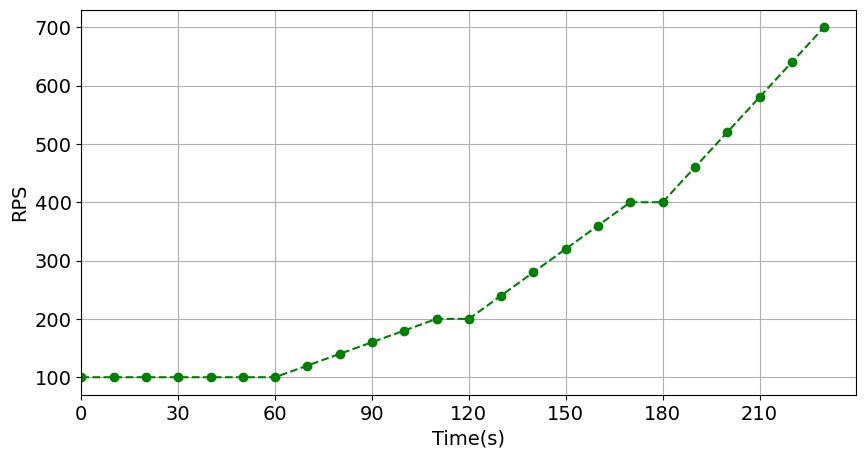
\includegraphics[width=4.3cm]{images/evaluation/linear_test_workload.png}
        \caption{Linear}
        \label{fig:test workloads linear}
    \end{subfigure}
    \begin{subfigure}{4.3cm}
        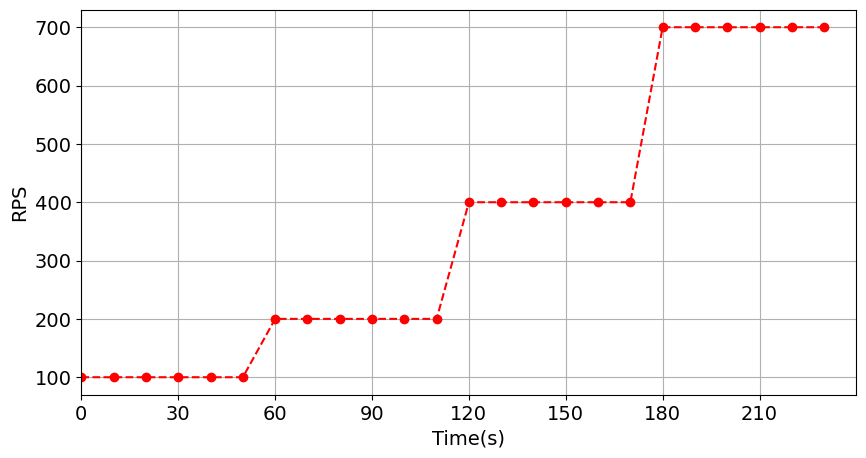
\includegraphics[width=4.3cm]{images/evaluation/spike_test_workload.png}
        \caption{Spike}
        \label{fig:test workloads spike}
    \end{subfigure}
    \caption{Test workloads}
    \label{fig:test workloads}
\end{figure}



실험은 HPA의 default와 optimal 그리고 UHPA 총 세 가지 모드를 활용합니다. 각 모드마다 각 test workload별로 15번씩 실행하여 총 90번의 실험을 진행했습니다. 외부 변수를 줄이기 위해 Kind cluster는 매 실험마다 새로 구축됩니다. Cluster 구축이 완료되고 각 모드별 세팅이 완료되면 랜덤한 시점에 wrk2 tool을 이용하여 traffic을 부과합니다. 성능 평가를 위한 지표로 매 실험의 끝에 각 서비스 별 증가한 pod 수를 모니터링하고 workload에서 발생된 총 requests 수와 2xx responses 수의 비율인 HTTP request success ratio를 구합니다.

먼저 각 모드별 스케일링 성능을 비교합니다. 우리는 social nerwork application의 11개 stateless 서비스 중 test workload에 의해 pod의 수가 증한 6개 마이크로서비스(compose-post, home-timeline, post-storage, text, user-mention, user-timeline)에 대한 결과를 확인하였습니다. Fig. \ref{fig:test workloads}는 각 test workload에서 실험 종료 후 limits.cpu 값에 따라 최종 pod의 개수를 나타냅니다. 모든 값은 15번 진행된 테스트의 평균 값입니다.

Default HPA는 두 모드 대비 상대적으로 낮은 스케일링 성능을 보여줍니다. 이는 Section {sec:background and motivation}에서 분석한 것처럼 긴 scrape interval에 의해 현재 CPU 사용량을 감지하는데 너무 오랜 시간이 걸리기 때문입니다. Optimal HPA는 조금 더 좋은 성능을 보여주며 특히 x2.5 limits.cpu에서 일부 마이크로서비스에서 UHPA와 비슷한 수준의 스케일링 성능을 확인할 수 있습니다. 하지만 x2.5 limits.cpu를 제외한 대부분은 여전히 UHPA 대비 현저히 떨어지는 스케일링 성능을 보여줍니다. 이는 메트릭서버가 간격을 두고 수집된 두 CPU 사용량의 평균을 사용함으로 현재 CPU 사용량을 과소평가하기 때문입니다. 이러한 문제는 Spike workload에서 더 두드러지게 나타납니다.

모든 테스트에서 UHPA가 HPA의 두 모드 대비 우월한 스케일링 성능을 보여 주며 특히,  x1.5 limits.cpu부터 HPA의 두 모드와 확연한 차이를 드러냅니다. 준수한 성능을 보이는 Optimal HPA의 x2.5 limits.cpu도 대부분의 서비스가 UHPA의 x1.5 또는 x.2.0 limits.cpu와 비슷하게 스케일링됩니다. 또한 UHPA는 신속한 CPU 사용량 감지로 linear workload와 spike workload 간의 스케일링 성능 간 큰 차이가 없습니다.

다음으로 스케일링 성능이 시스템 QoS에 미치는 영향을 비교합니다. Table \ref{tab:success ratio}은 limits.cpu 값에 따른 각 모드별 request success ratio를 보여줍니다. 동일한 limits.cpu에서 스케일링 성능이 다른 각 모드 별로 request success ratio에서 상당한 차이를 나타냅니다. 이 결과는 스케일링 성능이 실제 시스템의 QoS에 미치는 영향이 상당히 크다는 것을 증명합니다. 스케일링성능이 좋은 UHPA는 두 모드 대비 항상 높은 request success ratio을 보여줍니다. 또한, UHPA는 x1.0 limits.cpu을 제외하고 각 한 단계 낮은 limits.cpu에서 optimal HPA의 결과와 비슷하거나 우월한 성능을 나타냅니다.  스케일링 성능과 마찬가지로 spike workload에서 UHPA는 다른 두 모드와 더 큰 격차를 보여줍니다. UHPA는 spike workload의 x2.5 limits.cpu에서 default 모드 대비 최대 93\% 우수한 request success ratio를 보여줍니다.

\begin{figure}[tb]
    \begin{subfigure}{.48\textwidth}
        \centering
        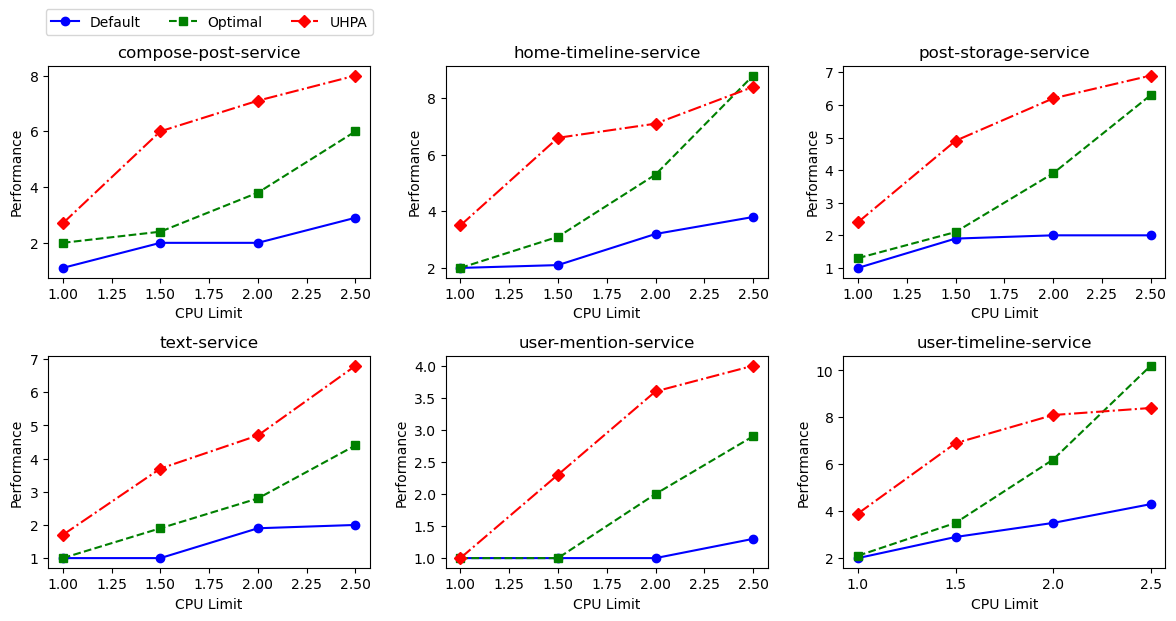
\includegraphics[width=1\linewidth]{images/evaluation/linear_result.png}
        \caption{Linear workload}
        \label{fig:num of pods linear}
    \end{subfigure}
    \begin{subfigure}{.48\textwidth}
        \centering
        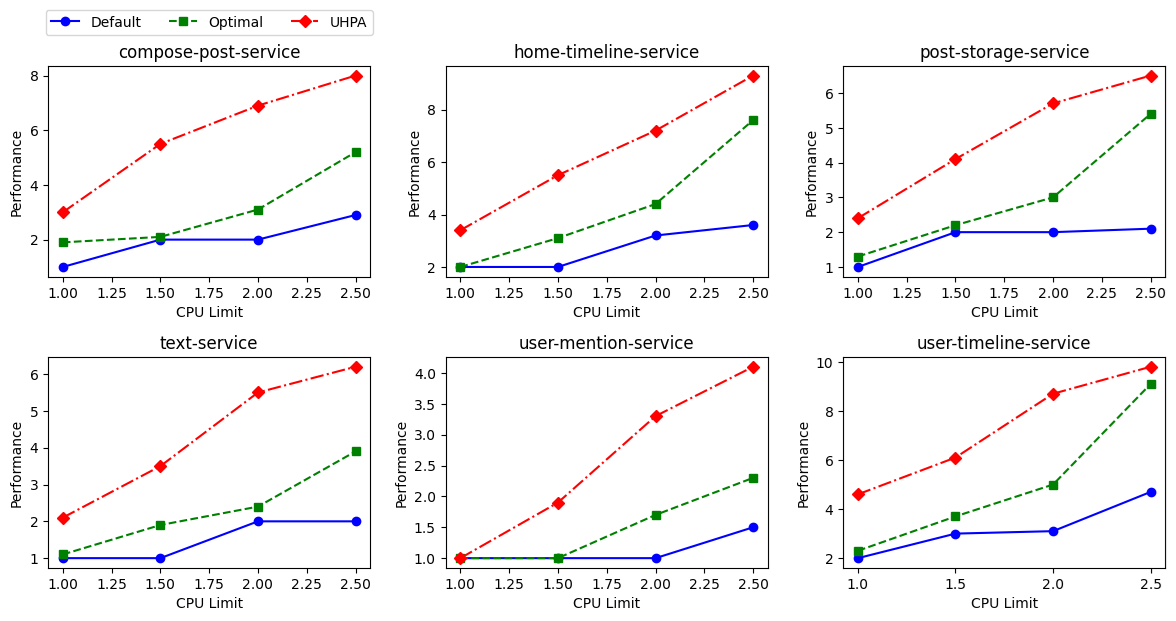
\includegraphics[width=1\linewidth]{images/evaluation/spike_result.png}
        \caption{Spike workload}
        \label{fig:num of pods spike}
    \end{subfigure}

    \caption{Number of pods according to CPU limit}
    \label{fig:num of pods}
\end{figure}

\begin{table}[tb]
    \centering
    \begin{tabular}{c|ccc|ccc}
        \noalign{\smallskip}\noalign{\smallskip}\hline\hline
        \multirow{2}{*}{\makecell{CPU                              \\Limit}} & \multicolumn{3}{c|}{Linear} & \multicolumn{3}{c}{Spike} \\
        \cline{2-7}
             & Default & Optimal & UHPA & Default & Optimal & UHPA \\
        \hline
        x1.0 & 22\%    & 26\%    & 34\% & 17\%    & 20\%    & 30\% \\
        x1.5 & 36\%    & 44\%    & 64\% & 28\%    & 33\%    & 48\% \\
        x2.0 & 47\%    & 64\%    & 85\% & 37\%    & 47\%    & 72\% \\
        x2.5 & 57\%    & 84\%    & 94\% & 46\%    & 68\%    & 89\% \\
        \hline
        \hline
    \end{tabular}
    \caption{Request success ratio}
    \label{tab:success ratio}
\end{table}

\begin{table}[ht]
    \caption{Resource Usage of UHPA Components}
    \begin{center}
        \begin{tabular}{|c|c|c|c|c|}
            \hline
            \multirow{2}{*}{\makecell{\textbf{Pods}}} & \multicolumn{2}{c|}{\textbf{Agent}} & \multicolumn{2}{c|}{\textbf{Controller}}                                         \\
            \cline{2-5}
                                                      & \textbf{CPU(m)}                     & \textbf{Memory(MB)}                      & \textbf{CPU(m)} & \textbf{Memory(MB)} \\
            \hline
            10                                        & 15                                  & 9                                        & 2               & 62                  \\
            \hline
            30                                        & 29                                  & 15                                       & 2               & 62                  \\
            \hline
            50                                        & 65                                  & 19                                       & 2               & 62                  \\
            \hline
            100                                       & 177                                 & 20                                       & 2               & 62                  \\
            \hline
        \end{tabular}
        \label{tab:system overhead}
    \end{center}
\end{table}

\subsection{System Overhead}
마지막으로 UHPA의 Agent와 Controller가 사용하는 리소스의 양을 확인하여 시스템 오버헤드를 조사했습니다. 실험을 위해 우리는 각 1개의 master node와 worker node를 구성하고 UHPA Agent와 Controller 각 1개씩 배포했습니다. Kubernetes는 노드당 최대 110개의 Pod를 지원하므로\cite{KubernetesLargeClusterBestPractices} 테스트용 nginx pod를 10에서 100개까지 배포하여 실험을 수행했습니다.  우리는 pod 수를 변경하면서 CPU 및 메모리 사용량을 지속적으로 모니터링했습니다.

표 \ref{tab:system overhead}는 pod 수가 10, 30, 50, 100개로 증가했을 때의 UHPA Agent 및 Controoler의 총 CPU 및 메모리 사용량을 보여줍니다. UHPA Agent의 평균 리소스 사용량은 pod 수에 따라 선형적으로 증가합니다. 100개 pod를 배포할 때 약간 더 높아지는 경향이 있지만 pod당 약 1.8m의 CPU 사용량은 충분히 허용 가능한 값이며, 이 값은 16개 코어가 있는 노드의 전체 CPU 리소스의 약 1\%에 해당됩니다. 반면에 UHPA 컨트롤러의 CPU 사용량은 최대 1초마다 스케일링 노티피케이션을 보내는 UHPA Agent 수에 영향을 받기 때문에 pod 수에 관계없이 안정적으로 유지됩니다. 10개의 UHPA Agent를 배포한 다른 실험에서 UHPA 컨트롤러는 에이전트당 2m 미만인 19m의 무시할만한 CPU를 사용합니다. 메모리 측면에서 UHPA 에이전트 및 컨트롤러는 영구적으로 관리하는 데이터가 없기 때문에 극소량의 메모리를 사용합니다. 실험 결과는 UHPA가 시스템에 미치는 영향이 충분히 허용 가능함을 보여줍니다.

% ----------------------------------------------------------------------------


\section{Conclusion}
본 연구에서는 Kubernetes의 기존 자동 스케일링 방식의 구조적 한계로 인한 스케일링 성능 저하를 확인하였습니다. 우리는 2단계 결정 메커니즘을 활용한 업스트림 기반의 자동 스케일러인 UHPA를 제안합니다. 실험 결과에 따르면 UHPA는 HPA의 기본 모드 대비 스케일링 속도를 약 20배 향상시켰고, 요청 응답률을 약 2배 높인 것으로 나타났습니다. 우리는 본 연구가 향후 실시간 수요 변화에 민감한 마이크로서비스의 신뢰성 향상에 기여할 것으로 기대합니다.


% ----------------------------------------------------------------------------


\bibliographystyle{plain}
\bibliography{references}

\vspace{12pt}
\end{document}